\colorlet{outlinecolor}{brightpurple}

\colorlet{headercolor}{outlinecolor}
\colorlet{rowcolor1}{outlinecolor!70}
\colorlet{rowcolor2}{outlinecolor!50}

\begin{tikzpicture}
	\node [mybox, fill=boxcolor, draw=outlinecolor] (box){%
		\begin{minipage}{0.3\textwidth}
			\vspace{0.1cm}
			
			\underline{Introduction}: It's a best practice to create all your changes on \textcolor{outlinecolor}{feature (or topic) branches}, make sure these changes stable, and then merge into the \inlinebash{main} branch.
		
			
			%			\begin{minipage}{\textwidth}
				%				\centering
				%%				\vspace{-2mm}
				%				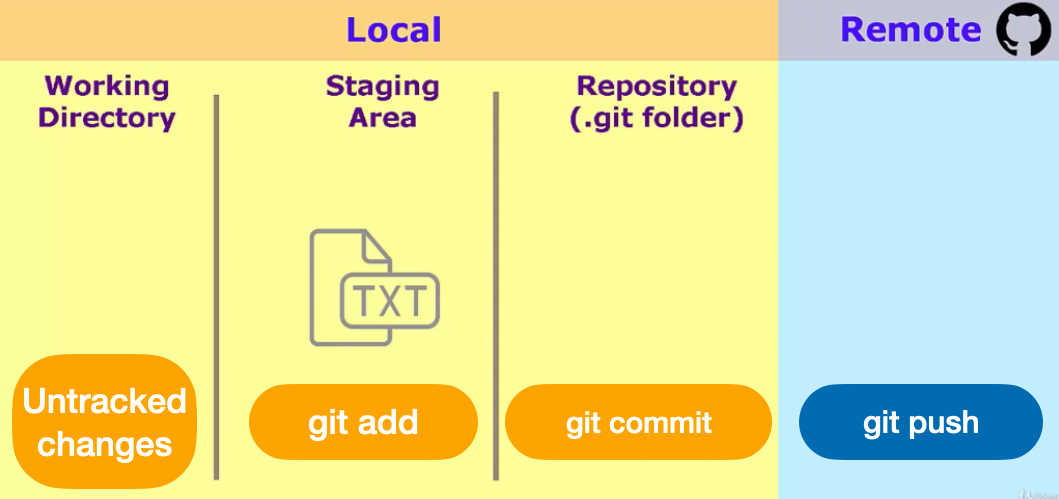
\includegraphics[width=0.5\textwidth]{images/git_stages.png}
				%				\vspace{-2mm}
				%				\captionof{figure}{Git states and associated commands. \href{https://www.udemy.com/course/git-complete/}{ \faLink{}  Source}}
				%			\end{minipage}
			
		\end{minipage}
	};
	\node[fancytitle, right=10pt, fill=outlinecolor, text=background, draw=outlinecolor, rounded corners] at (box.north west) {Branches};
\end{tikzpicture}